% Insert in the relevant Methods subsection; compile from overleaf/SWBAM/.
\begin{figure*}[!t]
    \centering
    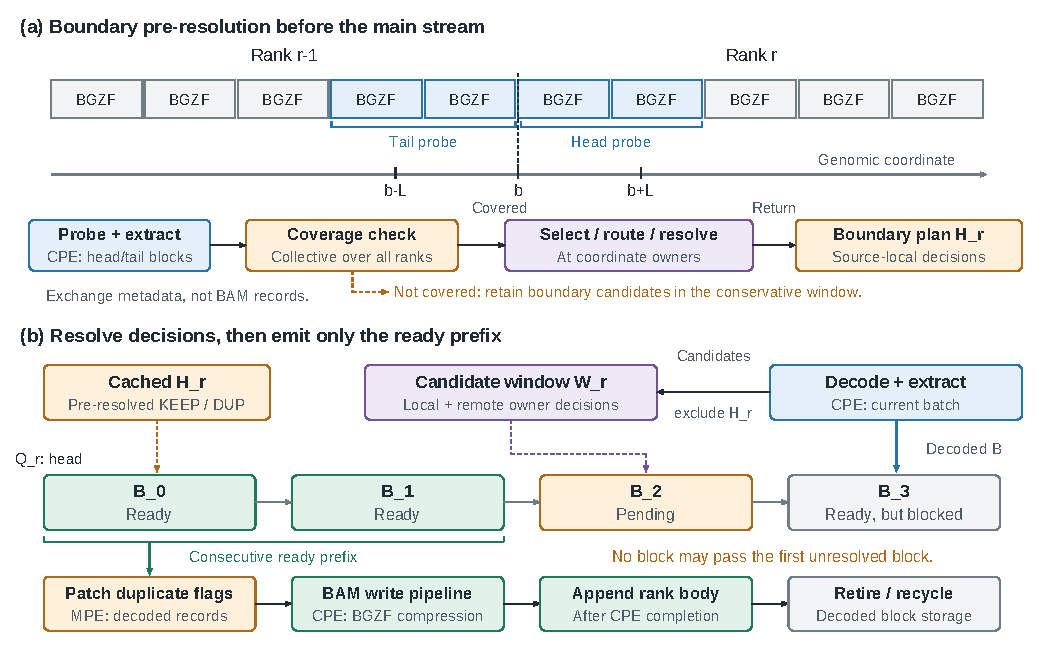
\includegraphics[width=\textwidth]{../figs/swbam_markdup_boundary.pdf}
    \caption{Boundary resolution and ordered emission in one-pass
    distributed duplicate marking. (a) Head/tail BGZF blocks are probed before
    the main stream. For a boundary $b$ on the same reference, the probe must
    cover the required $b-L$ and $b+L$ limits; coverage is checked collectively.
    Covered boundary candidates are routed to their coordinate owners and
    resolved, with source-local decisions cached in $H_r$. Insufficient
    coverage selects conservative boundary retention. (b) Pre-resolved
    candidates are excluded from ordinary window processing. Decisions from
    $H_r$ and the candidate window update retained decoded blocks in $Q_r$.
    Only a consecutive ready prefix may be patched, compressed, appended and
    retired. Solid arrows show data/order dependencies; dashed arrows show
    fallback or decision updates. Boundary probing entails extra decoding.}
    \label{fig:swbam_markdup_boundary}
\end{figure*}
